\chapter{Аудиоинтерфейс ostis-систем}
\chapauthortoc{Захарьев В.А.\\Азаров И.С.\\Вашкевич М.И.\\Крищенович В.А.\\Жаксылык К.}
\label{chapter_audio_interfaces}

\vspace{-7\baselineskip}

\begin{SCn}
\begin{scnrelfromlist}{авторы}
    \scnitem{Захарьев В.А.}
    \scnitem{Азаров И.С.}
    \scnitem{Вашкевич М.И.}
    \scnitem{Крищенович В.А.}
    \scnitem{Жаксылык К.}
\end{scnrelfromlist}

\bigskip

\scntext{аннотация}{Данная глава посвящена рассмотрению вопросов создания \textit{аудио} и \textit{речевых интерфейсов} для \textit{интеллектуальных компьютерных систем нового поколения}. Предлагается использование подхода на основе онтологического проектирования и формализации системы понятий из предметной области аудиоинтерфейсов, посредством \textit{Технологии OSTIS}. Изложены основные идеи, лежащие в основе данного подхода, а также их отличительные особенности от общепринятых. Показано, что в перспективе использование данного подхода может обеспечить свойства \textit{унификации}, \textit{семантической совместимости} и \textit{интероперабельности}, при разработке аудио и речевых интерфейсов, что в итоге позволит существенным образом сократить издержки при создании \textit{интеллектуальных компьютерных систем нового поколения} для решении \textit{комплексных задач}.}

\bigskip

\begin{scnrelfromlist}{подраздел}
    \scnitem{\ref{sec_audio_interfaces_review}~\nameref{sec_audio_interfaces_review}}
    \scnitem{\ref{sec_audio_interfaces_ostis_approach}~\nameref{sec_audio_interfaces_ostis_approach}}
    \scnitem{\ref{sec_audio_interfaces_subject_area_problems}~\nameref{sec_audio_interfaces_subject_area_problems}}
    \scnitem{\ref{sec_audio_interfaces_subject_area_signal_models}~\nameref{sec_audio_interfaces_subject_area_signal_models}}
    \scnitem{\ref{sec_audio_interfaces_conclusion}~\nameref{sec_audio_interfaces_conclusion}}
\end{scnrelfromlist}

\bigskip

\begin{scnrelfromlist}{ключевое понятие}
    \scnitem{сигнал}
    \scnitem{аудиосигнал}
    \scnitem{речевой сигнал}
    \scnitem{модель сигнала}
    \scnitem{аудиоинтерфейс}
    \scnitem{речевой интерфейс}
\end{scnrelfromlist}

\bigskip

\begin{scnrelfromlist}{библиографическая ссылка}
    \scnitem{\scncite{Pearl2016}}
    \scnitem{\scncite{Chen2021audio}}
    \scnitem{\scncite{Lu2002content}}
    \scnitem{\scncite{Fernandes2022}}
    \scnitem{\scncite{Popov2020interspeech}}
    \scnitem{\scncite{Povey2011ASRU}}
    \scnitem{\scncite{Deepa2021}}
\end{scnrelfromlist}

\end{SCn}


\section{Введение в \textit{Главу \ref{chapter_audio_interfaces}~\nameref{chapter_audio_interfaces}}}
\label{sec_audio_interfaces_review}

Разговорная речь является одной из наиболее естественных и эффективных форм передачи информации между людьми. Этот факт объясняет значительный интерес исследователей к вопросам развития и применения \textit{речевых интерфейсов} для обеспечения человеко-машинного взаимодействия в составе современных коммуникационных, мультимедийных и интеллектуальных систем (см. \scncite{Pearl2016}, \scncite{Chen2021audio}).

Более всеобъемлющей формой обеспечения взаимодействия с пользователем и окружающей средой посредством анализа и синтеза акустических сигналов является \textit{аудиоинтерфейс}. Данную разновидность интерфейса, выступающей родительской по отношению к речевым, можно кратко определить как аппаратно-программный комплекс осуществляющий анализ и синтез сигналов во всем доступном спектре параметров носителей акустической информации. Например, для решения задач анализа обстановки и событий происходящих в акустическом окружении системы, синтеза неречевых сигналов (звуков техногенного и природного характера, сигналов оповещения, музыки, и так далее) (см. \scncite{Lu2002content}).

Об актуальности направления разработки аудио и речевых интерфейсов свидетельствуют следующие основные тенденции развития данного направления:
\begin{textitemize}    
    \item экономические показатели и прогнозы развития рынка речевых технологий, текущие среднегодовые темпы роста которого, по оценкам экспертов, составляют порядка 22\%, а совокупный объем будет равен 59,6 млрд. долл. США к 2030 (см. \scncite{Fernandes2022});
    \item появление широкого спектра продуктов на основе речевого интерфейса, получивших массовое распространение. В первую очередь это персональные голосовые ассистенты, такие как  ``Alexa'' (Amazon), ``Siri'' (Apple), ``Сortana'' (MicroSoft), ``Алиса'' (Yandex) (см. \scncite{Bellegarda2014}, \scncite{Lemley2017}, \scncite{Hoy2018});
    \item интерес со стороны научного сообщества, выражающийся в росте публикаций в этом направлении исследований на 15\% за последние 5 лет (см. \scncite{Semscholar2022stat}).
\end{textitemize}

Необходимо отметить, что основная масса научных публикаций в данном направлении посвящена развитию базовых технологий, являющихся составляющими речевого интерфейса, таким как синтез речи по тексту, а также распознавание речи в текст (см. \scncite{Popov2020interspeech}, \scncite{Povey2011ASRU}, \scncite{Deepa2021}). Последние достижения в этих направлениях связаны с бурным развитием нейросетевых моделей и вычислительных средств. Они позволили довести качественные характеристики использования речевых технологий до коммерческого уровня (см. \scncite{Vosk2021}, \scncite{Radford2022robust}).

Большинство существующих систем, как правило, рассчитаны на решение определенного круга задач и сложно совместимы друг с другом. Данный факт в особенности остро проявляется при проектировании сложных систем, наподобие интеллектуальных персональных диалоговых ассистентов (см. \textit{\nameref{fig:speech-hmi-components}}), требующих использования многообразия различных видов обрабатываемой информации и различных \textit{моделей решения задач}. Такие системы, кроме стандартных модулей распознавания (ASR, automatic speech recognition) и синтеза (TTS, text to speech), на уровне аудиоинтерфейса также должны содержать модели, определяющие наличие/отсутствие речи в аудиосигнале в сложной акустической обстановке, классификации звуков окружающей среды, распознавание диктора и пр. Помимо этого элементы речевого интерфейса должны быть совместимы с более высокоуровневыми модулями обработки естественно-языковой информации, такими как модули понимания (SLU, spoken language understanding) и генерации речи (SLG, spoken language generation), управления диалогом (DM, dialog manager) (см. \scncite{Delic2019speech}). 

\begin{figure}[H]
    \centerline{
        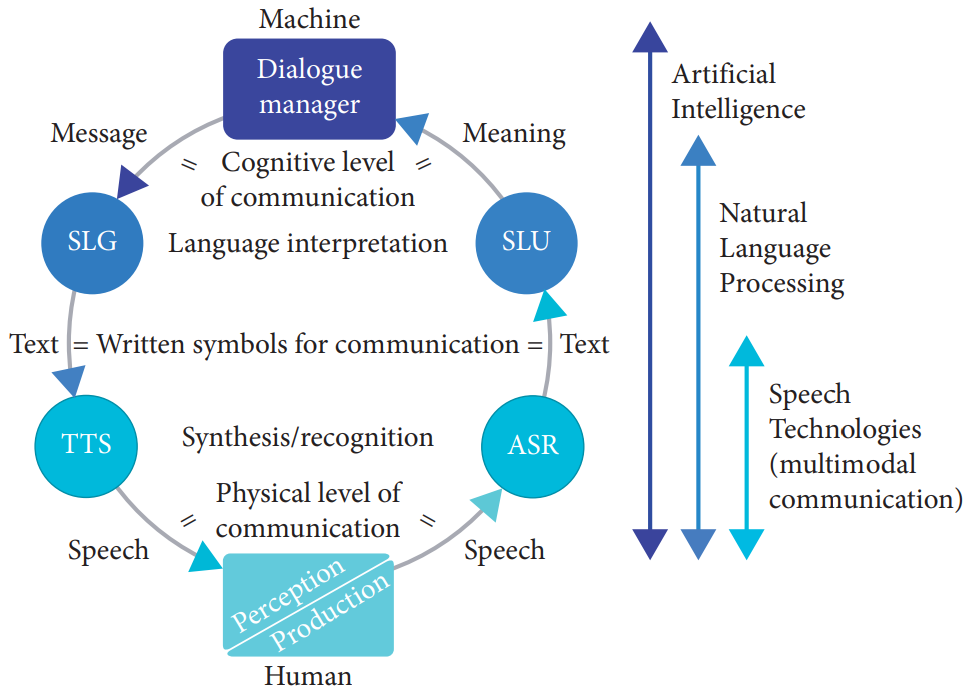
\includegraphics[scale=0.6, width=0.6\textwidth]{author/part4/figures/ch43_fig01_speech-hmi-components.png}
    }
    \caption{Компоненты системы человеко-машинного речевого диалога \cite{Delic2019speech}}
    \label{fig:speech-hmi-components}
\end{figure}

Всё это требует разработки подходов, основанных не только на методах машинного обучения и обработке сигналов, но и на обработке естественного языка, символических методах искусственного интеллекта, онтологическом проектировании и формализации предметной области аудиоинтерфейса. Это позволит создать системы, которые обладают полным спектром знаний в формализованном виде о типах задач, которые они должны решать, и методах, доступных для их решения.

Необходимым условием для создания таких систем нового поколения, обладающих улучшенными характеристиками по критериям \textit{интероперабельности} и \textit{гибкости} является также тот факт, что данные системы должны быть построены на основе базовой технологии, позволяющей обеспечить такое единство формы представления информации на всех её уровнях.
 
Совокупность данных факторов приводит к необходимости создания \textit{интеллектуальных компьютерных систем нового поколения}, которые будут включать в себя модули аудио и речевого интерфейса, построенные на основе принципов интероперабельности и семантической совместимости для решения \textit{комплексных задач}.


\section{Применение принципов онтологического проектирования при разработке аудиоинтерфейсов}
\label{sec_audio_interfaces_ostis_approach}

Для достижения поставленной цели предлагается прибегнуть к подходу на основе принципов, лежащих в основе ``Стандарта открытой технологии онтологического проектирования, производства и эксплуатации семантически совместимых гибридных интеллектуальных компьютерных систем'' или кратко ``Стандарта технологии OSTIS'' (см. \scncite{Standart2021}).

Суть подхода заключается в рассмотрении процесса проектирования аудиоинтерфейса как интерфейсной подсистемы в рамках общего процесса разработки \textit{интеллектуальной компьютерной системы} и построении её формальной \textit{логико-семантической модели}.

Для создания подобной модели интеллектуальной компьютерной системы нового поколения необходимо:
\begin{textitemize}    
    \item произвести декомпозицию информационной компьютерной системы на компоненты. Качество декомпозиции при этом определяется простотой последующего синтеза общей формальной модели из формальных моделей выделенных компонентов.
    \item провести \textit{конвергенцию} выделенных компонентов в целях построения совместимых (легко интегрируемых) формальных моделей этих компонентов;
    \item провести интеграцию построенных формальных моделей выделенных компонентов и получить общую \textit{формальную модель}.
\end{textitemize}

В качестве технологической основы для реализации предлагаемого подхода будет использоваться Технология OSTIS (см. \scncite{Standart2021}), соответственно подсистема аудиоинтерфейса будет строиться как \textit{многократно используемый компонент}, который в будущем будет при необходимости встраиваться в различные ostis-системы.

Ориентация на \textit{Технологию OSTIS} обусловлена ее следующими основными преимуществами:
\begin{textitemize}
\item в рамках указанной технологии предложены унифицированные средства представления различных видов знаний, в том числе --- \textit{метазнаний}, что позволяет описать всю необходимую для анализа информацию в одной базе знаний в едином ключе (см. \scncite{Davydenko2017});
\item используемый в рамках технологии формализм позволяет специфицировать в базе знаний не только понятия, но и любые внешние с точки зрения базы знаний файлы (например, фрагменты речевого сигнала), в том числе --- синтаксическую структуру таких файлов;
\item предложенный в рамках технологии подход к представлению различных видов знаний (см. \scncite{Davydenko2017}) и моделей их обработки (см. \scncite{Shunkevich2018}) обеспечивает модифицируемость ostis-систем, то есть позволяет легко расширять функциональные возможности системы, вводя новые виды знаний (новые системы понятий) и новые модели обработки знаний;
\end{textitemize}

Более подробно принципы построения комплексной технологии разработки и поддержки жизненного цикла \textit{интеллектуальных компьютерных систем нового поколения} --- \textit{Технологии OSTIS} --- изложены в \textit{Главе \ref{chapter_new_generation_systems}~\nameref{chapter_new_generation_systems}}.

В данной главе монографии, в отличие от предыдущих работ авторов, посвященных вопросам семантического анализа голосовых сообщений на основе формализованного контекста и создания диалоговых ассистентов на основе модели ментального лексикона или мультимодальной системы на основе нейросимволического подхода, Технология OSTIS используется для непосредственного построения онтологии подсистем аудио интерфейса (см. \scncite{Zahariev2018}, \scncite{Zahariev2019}, \scncite{Zahariev2020}, \scncite{Zahariev2021}).

Поскольку \textit{аудиоинтерфейс} \textit{интеллектуальных компьютерных систем нового поколения} должен иметь архитектуру, соответствующую общим правилам построения ostis-систем, можно выделить и формализовать следующие основные его части: 
\begin{SCn}
	\scnheader{аудиоинтерфейс \textit{интеллектуальных компьютерных систем нового поколения}}
	\scntext{сокращение}{аудиоинтерфейс \textit{интеллектуальных компьютерных систем}}
	\begin{scnrelfromset}{обобщенная декомпозиция}
		\scnitem{база знаний подсистемы аудиоинтерфейса \textit{интеллектуальных компьютерных систем нового поколения}}
		\scnitem{решатель задач подсистемы аудиоинтерфейса \textit{интеллектуальных компьютерных систем нового поколения}}
		\scnitem{интерфейс для взаимодействия с остальными интерфейсными подсистемами ostis-системы}
	\end{scnrelfromset}
\end{SCn}

Согласно общим принципам организации интерфейсов ostis-систем, изложенным в \textit{Главе \ref{chapter_interfaces}}, \textit{аудио- и речевой интерфейс} относятся к подмножеству \textit{SILK-интерфейсов} \textit{пользовательских интерфейсов} \textit{интеллектуальных компьютерных систем}. 

Для решения задачи построения пользовательского интерфейса в базе знаний пользовательского интерфейса ostis-системы необходимо наличие \textit{sc-модели} компонентов \textit{пользовательского интерфейса}, интерфейсных действий пользователей, а также классификации пользовательских интерфейсов в целом. При проектировании интерфейса используется компонентный подход, который предполагает представление всего интерфейса приложения в виде отдельных \textit{специфицированных компонентов}, которые могут разрабатываться и совершенствоваться независимо.

Таким образом, необходимо отметить, что процесс разработки аудиоинтерфейса для \textit{интеллектуальных компьютерных систем нового поколения}, подразумевает прежде всего создание семантически структурированных баз знаний в виде иерархической системы предметных областей и соответствующих им онтологий, специфицирующих эти предметные области. Следовательно, первым шагом для достижения поставленной цели должен являться этап выделения и формализации сущностей аудио и речевого интерфейса для погружения данной информации в базу знаний интеллектуальной компьютерной системы.

С нашей точки зрения можно провести декомпозицию предметных областей и онтологий, входящих в \textit{базу знаний} \textit{аудиоинтерфейса}, по следующим основным направлениям:

\begin{SCn}
	\scnheader{Предметная область и онтология аудиоинтерфейса интеллектуальных компьютерных систем нового поколения}
	\begin{scnreltoset}{декомпозиция}
		\scnitem{Предметная область и онтология задач аудиоинтерфейса}
		\scnitem{Предметная область и онтология моделей параметрического представления сигнала}
	\end{scnreltoset}
\end{SCn}

Как видно, во главу онтологии положен функциональный подход к декомпозиции предметных областей, что является вполне естественным, поскольку соответствует природе задач, реализуемых аудиоинтерфейсом.

Представленные выше принципы в совокупности позволяют осуществлять конвергенцию и интеграцию компонентов как на уровне подсистемы аудиоинтерфейса, так и на уровне всей \textit{интеллектуальной компьютерной системы нового поколения} в целом, что, в свою очередь, позволяет перевести \textit{интеллектуальную информационную систему} в класс гибридных, \textit{интероперабельных} и \textit{семантически совместимых систем}.
  
 Далее перейдём непосредственно к рассмотрению конкретных предметных областей и построению онтологии аудиоинтерфейса.

\section{Предметная область и онтология задач аудиоинтерфейса ostis-систем}
\label{sec_audio_interfaces_subject_area_problems}

Первым шагом на пути к построению базы знаний подсистемы аудиоинтерфейса \textit{интеллектуальных компьютерных систем нового поколения} является формализация онтологии верхнего уровня. В основе данной онтологии предлагается положить формализованное представление основных сущностей предметной области и их свойств, а также функциональных задач, которые аудио и речевой интерфейс призваны решать. 

К основным сущностям, требующим формализации и погружения в базу знаний, относятся множества понятий, представленные далее. 

Одним из ключевых понятий, требующих формализации, является базовое определение самого сигнала, а также основных разновидностей сигналов, в зависимости от их природы представляющих наибольший интерес в области аудиоинтерфейсов. Чтобы сделать процесс описания средствами Технологии OSTIS более ясным, перед непосредственным переходом к нему приведем перечень основных сущностей и понятий, которые требуют формализации и погружения базу знаний:

\begin{textitemize}    
    \item сигнал;
    \item акустический сигнал;
    \item аудиосигнал;
    \item речевой сигнал.
\end{textitemize}

В зависимости от способа математического описания обрабатываемого сигнала в ostis-системе, можно определить следующие их классы:

\begin{textitemize}    
    \item аналоговый сигнал;
    \item дискретный сигнал;
    \item цифровой сигнал;
    \item периодический сигнал;
    \item апериодический сигнал;
    \item гармонический сигнал;
    \item тональный сигнал;
    \item шумовой сигнал;
    \item импульсный сигнал;
\end{textitemize}

Формализуем также основные понятия, связанные с характеристиками самого сигнала, по следующим основным его атрибутам \textit{\nameref{fig:speech-structure-segment-suprasegment}}:
\begin{textitemize}  
    \item амплитуда сигнала;
    \item частота сигнала;
    \item фаза сигнала;
    \item интенсивность сигнала;
    \item длительность сигнала;
    \item мощность/энергия сигнала;
    \item осцилограмма сигнала;
    \item спектр сигнала;
    \item частота дискретизации сигнала;
    \item степень квантования сигнала;
\end{textitemize}

\begin{figure}[H]
    \centerline{
        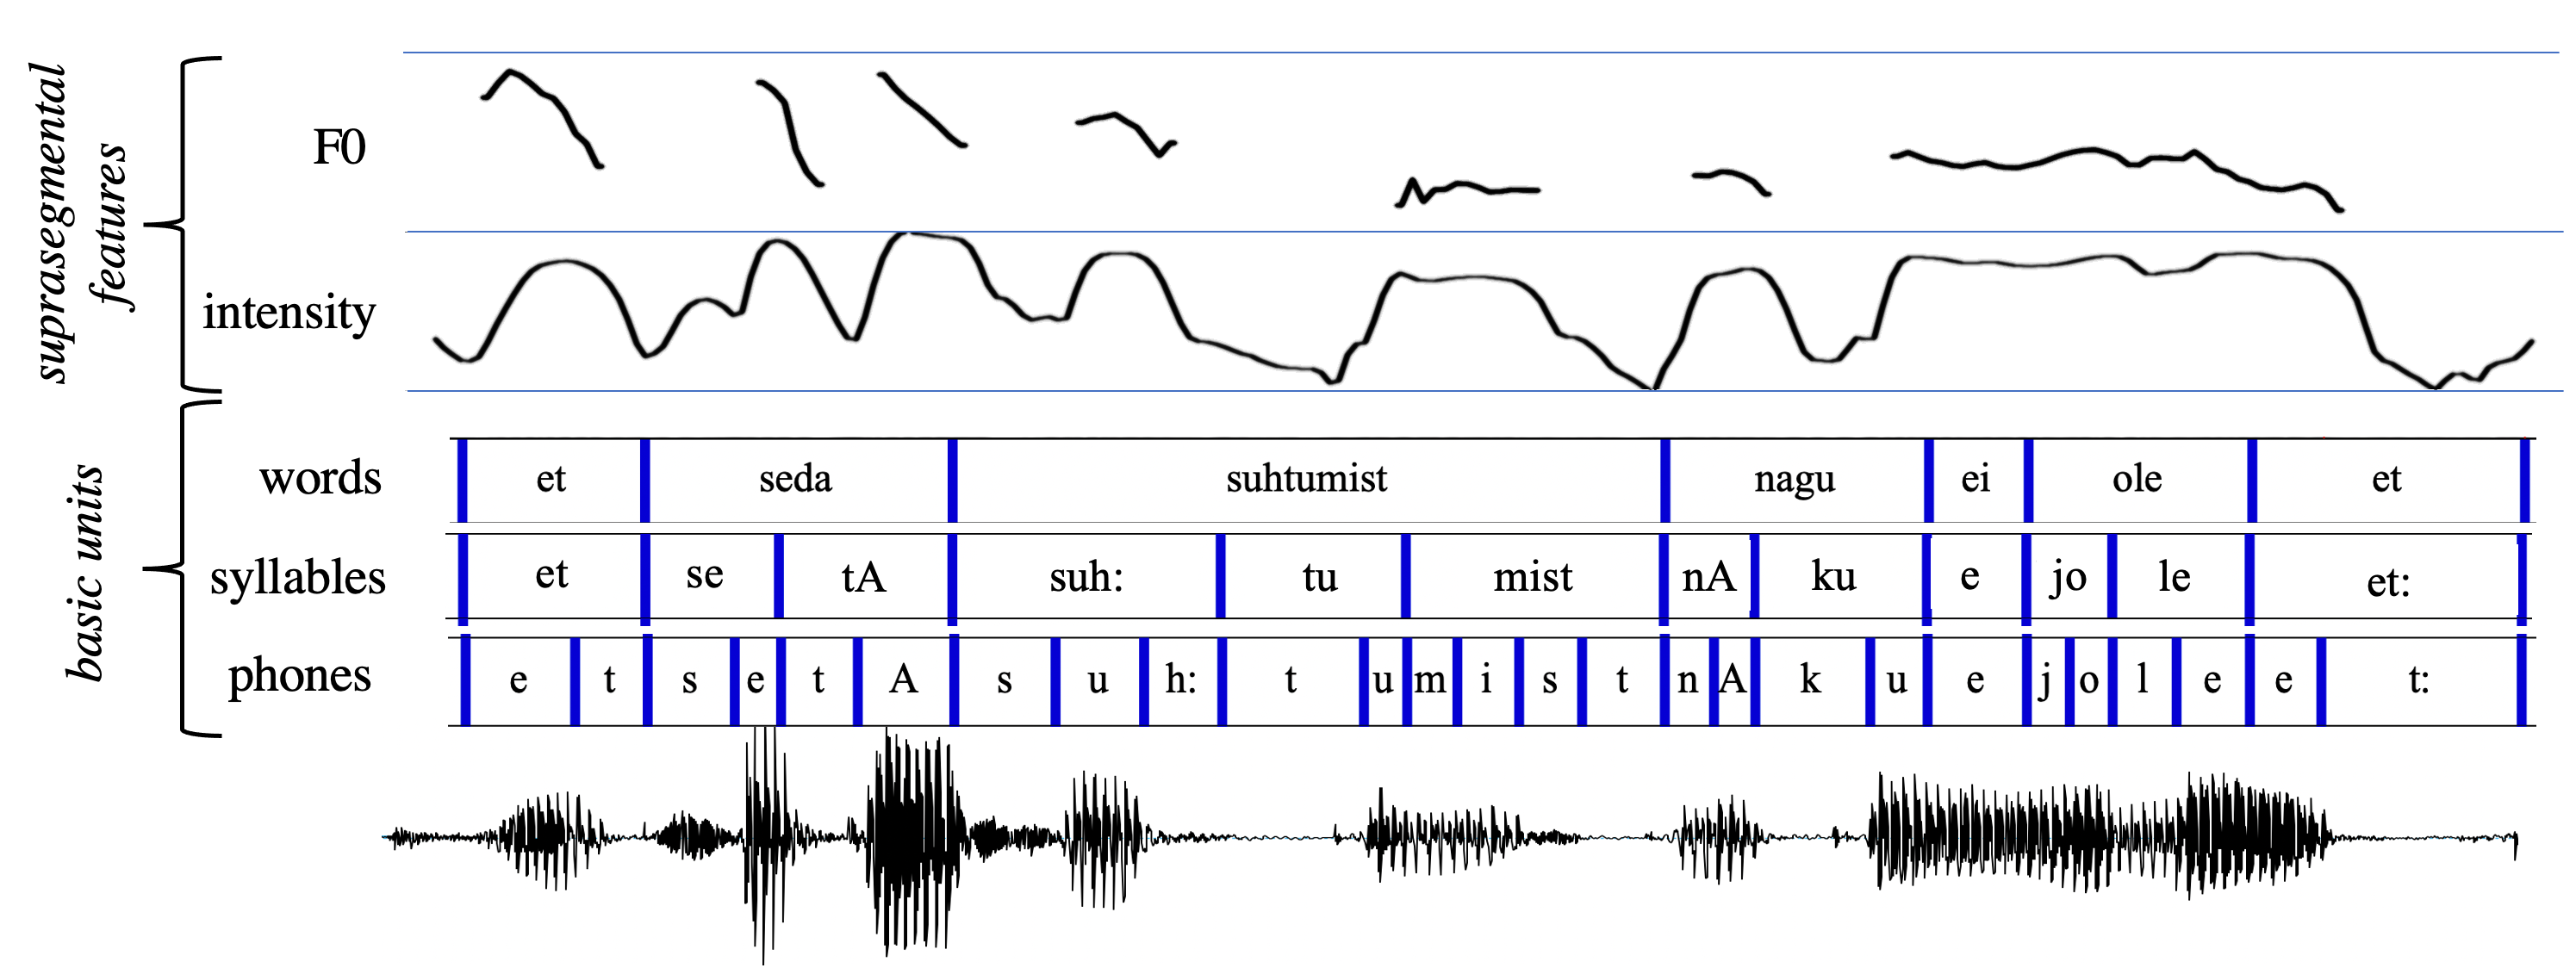
\includegraphics[scale=0.8, width=1.0\textwidth]{author/part4/figures/ch43_fig02_speech-structure-segment-suprasegment.png}
    }
    \caption{Сегментные и надсегментные характеристики речевого сигнала \cite{Okko2022}}
    \label{fig:speech-structure-segment-suprasegment}
\end{figure}

К ключевым понятиям предметной области, лежащим в семантической окрестности подпространства функционального назначения аудиоинтерфейсов и обработки аудиосигналов, относятся:
\begin{textitemize}    
    \item анализ аудиосигнала;
    \item синтез аудиосигнала;
    \item кодирование аудиосигнала;
    \item шумоочистка аудиосигнала;
    \item классификация аудиосигнала;
    \item классификация событий (Enviromental Sound Classification, Acoustic Scenes and Events);
    \item детектирование аномалий (Anomalous Sound Detection);
    \item идентификация положения источника в пространстве (Sound Source Localization);
\end{textitemize}

Основные понятия аудио и речевого интерфейса также тесно связаны с основными его характеристиками \textit{\nameref{fig:speech-structure-segment-suprasegment}}, которые можно разделить на следующие основные группы понятий:
\begin{textitemize}
    \item характеристики речевого сигнала;
    \item лингвистические характеристики сигнала;
    \item паралингвистические характеристики сигнала;
    \item экстралингвистические характеристики сигнала;
    \item сегментные характеристики речевого сигнала (Segmantal Features);
    \item надсегментные характеристики речевого сигнала (Suprasegmental Features);
    \item громкость речевого сигнала;
    \item тембр речевого сигнала;
    \item темп речевого сигнала;
    \item частота основного тона сигнала;
    \item фонемный состав речевого сигнала.
\end{textitemize}


Основными понятиями предметной области, лежащими в семантической окрестности функционального назначения речевого сигнала и обработки аудиосигналов, являются следующие:
\begin{textitemize}    
    \item анализ речевого сигнала;
    \item детектирование наличия ключевых слов (Key Words Spotting);
    \item активация по ключевому слову (Wake Up Word Detection);
    \item детектирование наличия речевого сигнала (Voice Activity Detection);
    \item синтез речевого сигнала;
    \item синтез текста в речь (Text-to-Speech Synthesis);
    \item эмоциональный синтез текста в речь (Emotional Text-to-Speech Syntehsis);
    \item cинтез пения (Sing Synthesis);
    \item распознавание эмоций в речевом сигнале (Emotional Speech Recognition);
    \item распознавание диктора;
    \item сепарация речи (speech separation, speech diarization);
    \item классификация диктора (Speaker Recognition);
    \item верификация диктора (Speaker Verification);
\end{textitemize}

Необходимо отметить, что вышеобозначенные понятия зачастую сложным и нетривиальным образом связаны между собой в процессе перехода от источников информации к непосредственным физическим параметрам. Такую сложную структуру сигнала можно представить в виде схемы его информационной структуры \textit{\nameref{fig:speech-signal-inf-structure-ru}}. Этот факт требует от \textit{интеллектуальных компьютерных систем нового поколения} формализации понятий для того, чтобы система могла автоматически интерпретировать взаимосвязи между данными характеристиками при работе с аудио и речевыми сигналами. И, как следствие, выдать ответ пользователю, объясняющий на основе каких характеристик система пришла к тому или иному выводу. 

Поскольку для построения \textit{интеллектуальных компьютерных систем нового поколения} в фокусе лежат именно задачи, связанные с обработкой речевых сигналов, решение которых необходимо в первую очередь для построения речевого интерфейса, акцент при формализации постараемся сделать на особенности данной предметной области.

\begin{figure}[H]
    \centerline{
        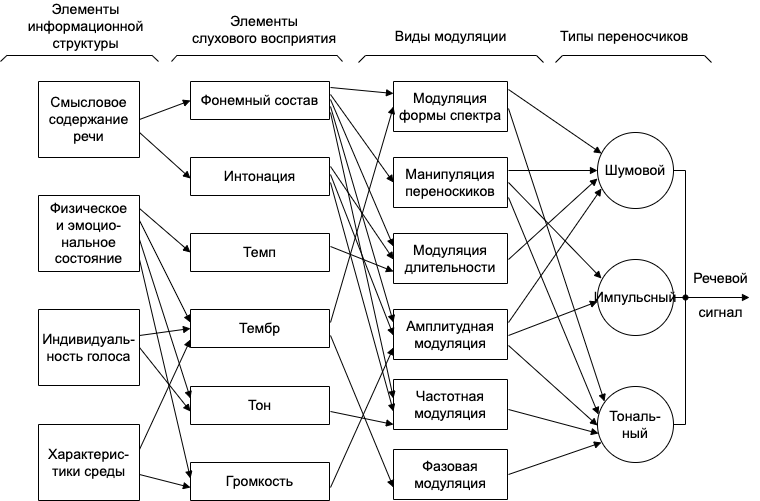
\includegraphics[scale=0.8, width=1.0\textwidth]{author/part4/figures/ch43_fig03_speech-signal-inf-structure-ru.png}
    }
    \caption{Информационная структура речевого сигнала \cite{Lobanov2006}}
    \label{fig:speech-signal-inf-structure-ru}
\end{figure}

Основу \textit{sc-модели базы знаний} составляет иерархическая система предметных областей и соответствующих им онтологий. Ниже показан верхний уровень иерархии части \textit{базы знаний}, относящейся непосредственно к аудио и речевым интерфейсам.

Приведём формализованное представление некоторых из обозначенных выше понятий:

\begin{SCn}
\scnheader{сигнал}
\scntext{определение}{физический процесс, несущий сообщение (информацию) о каком-либо событии, состоянии объекта наблюдения либо передающий команды управления, оповещения и так далее}
\scnsuperset{акустический сигнал}
\begin{scnindent}
    \scntext{определение}{сигнал, представляющий собой распространение упругих волн в газообразной, жидкой или твердой среде}
\end{scnindent}
\scnsuperset{аудиосигнал}
\begin{scnindent}
    \scnidtf{слышимый звуковой сигнал}
    \scntext{определение}{акустический сигнал, параметры которого находятся в пределах диапазона значений доступного для восприятия органами чувств человека}
    \scnsuperset{акустический сигнал}
    \scntext{примечание}{диапазон частот аудиосигнала лежит в интервале от 20 до 20 000 Гц.}
\end{scnindent}
\scnsuperset{речевой сигнал}
\begin{scnindent}
	\scntext{определение}{аудиосигнал, который образуется в результате прохождения воздушных потоков через речевой тракт человека. В результате всевозможных акустических преобразований происходит формирование различных звуков речи}
	\scnhaselement{устная речь}
	\scnhaselement{речеобразование}
	\scntext{примечание}{механизм речеобразования человека представляет собой акустическую трубу с динамически изменяющимися параметрами поперечного сечения, возбуждаемую либо квазипериодической последовательностью импульсов, генерируемых голосовыми связками, либо турбулентным потоком воздуха, проталкиваемого сквозь сужения, в разных местах речевого тракта}
\end{scnindent}
\end{SCn}
 
В зависимости от модели представления сигнала в ostis-системе также могут быть определены следующие описания основных видов сигналов, применение которых обосновано особенностями природы анализируемого сигнала, а также решаемой задачей анализа:

\begin{SCn}
\scnheader{математическая модель сигнала}
\begin{scnreltoset}{объединение}
    \scnitem{аналоговый сигнал}
	\begin{scnindent}
	\scntext{определение}{сигнал параметры которого можно измерить в любой момент времени}
    \scntext{определение}{сигнал, у которого каждый из представленных параметров описывается функцией времени и непрерывным множеством возможных значений}
    \end{scnindent}
    \scnitem{дискретный сигнал}
	\begin{scnindent}
	\scntext{определение}{сигнал, у которого хотя бы один из представленных параметров описывается конечным множеством возможных значений}
	\begin{scnreltoset}{объединение}
	    \scnitem{дискретный по времени}
        \scnitem{дискретный по амплитуде}
    \end{scnreltoset}
    \end{scnindent}
    \scnitem{цифровой сигнал}
	\begin{scnindent}
	\scntext{определение}{сигнал, у которого каждый из представляющих параметров описывается функцией дискретного времени и конечным множеством возможных значений}
	\begin{scnrelfromset}{включает}
    \scnitem{дискретный по времени сигнал}
    \scnitem{квантованный (дискретный) по амплитуде сигнал}
    \end{scnrelfromset}
    \end{scnindent}
	\scnitem{периодический сигнал}
	\scnitem{апериодический сигнал}
	\scnitem{тональный сигнал}
	\scnitem{гармонический сигнал}
	\scnitem{имульсный сигнал}
	\scnitem{шумовой сигнал}
\end{scnreltoset}
\end{SCn}

Необходимо отметить, что по причине ограничений на размер материала для характеристик аудиосигнала приведем только иерархию общей их взаимосвязи, поскольку семантика данных понятий вполне характерна и для других областей технических наук и не требует подробных примеров и пояснений. 

\begin{SCn}
\scnheader{характеристика аудиосигнала}
\begin{scnreltoset}{объединение}
	\scnitem{амплитуда сигнала}
	\scnitem{частота сигнала}
	\scnitem{фаза сигнала}
	\scnitem{интенсивность сигнала}
	\scnitem{длительность сигнала}
	\scnitem{мощность сигнала}
	\scnitem{спектр сигнала}
	\scnitem{осцилограмма сигнала}
	\begin{scnindent}
    \scntext{определение}{функция фиксирующая зависимость изменения характеристик сигнала (в первую очередь амплитуды) от времени}
    \end{scnindent}
	\scnitem{спектрограмма сигнала}
	\begin{scnindent}
    \scntext{определение}{функция, фиксирующая зависимость спектральной плотности мощности аудиосигнала от времени}
    \end{scnindent}
	\scnitem{частота дискретизации сигнала}
	\begin{scnindent}
    \scntext{определение}{значение частоты, с которой производилась дискретизация сигнала по времени в процессе аналогово-цифрового преобразования}
    \begin{scnreltoset}{типовые значения}
        \scnitem{8000 Гц}
    	\scnitem{16000 Гц}
    	\scnitem{22050 Гц}
    	\scnitem{44100 Гц}
    	\scnitem{48000 Гц}
    \end{scnreltoset}
    \end{scnindent}
	\scnitem{уровень квантования сигнала}
    \begin{scnindent}
    \scntext{определение}{допустимое количество дискретных уровней сигнала выраженное как степень двойки и применяемое в процессе квантования сигнала по уровню в процессе аналогово-цифрового преобразования}
    \begin{scnreltoset}{типовые значения}
        \scnitem{8 бит}
    	\scnitem{10 бит}
    	\scnitem{12 бит}
    	\scnitem{16 бит}
    	\scnitem{24 бита}
    \end{scnreltoset}
    \end{scnindent}
\end{scnreltoset}
\end{SCn}

Важным аспектом в процессе проектирования является формализация \textit{классов задач} аудиоинтерфейса, поскольку благодаря этим знаниям в интеллектуальной системе могут (и должны) применяться соответствующие методы обработки, в зависимости от типа решаемой задачи. Фрагмент онтологии верхнего уровня типовых \textit{задач} решаемых \textit{интеллектуальной компьютерной системой} в области обработки аудио- и речевых сигналов представлено на \textit{\nameref{fig:audio-and-speech-tasks-formalization-ru}} 

\begin{figure}[H]
    \centerline{
        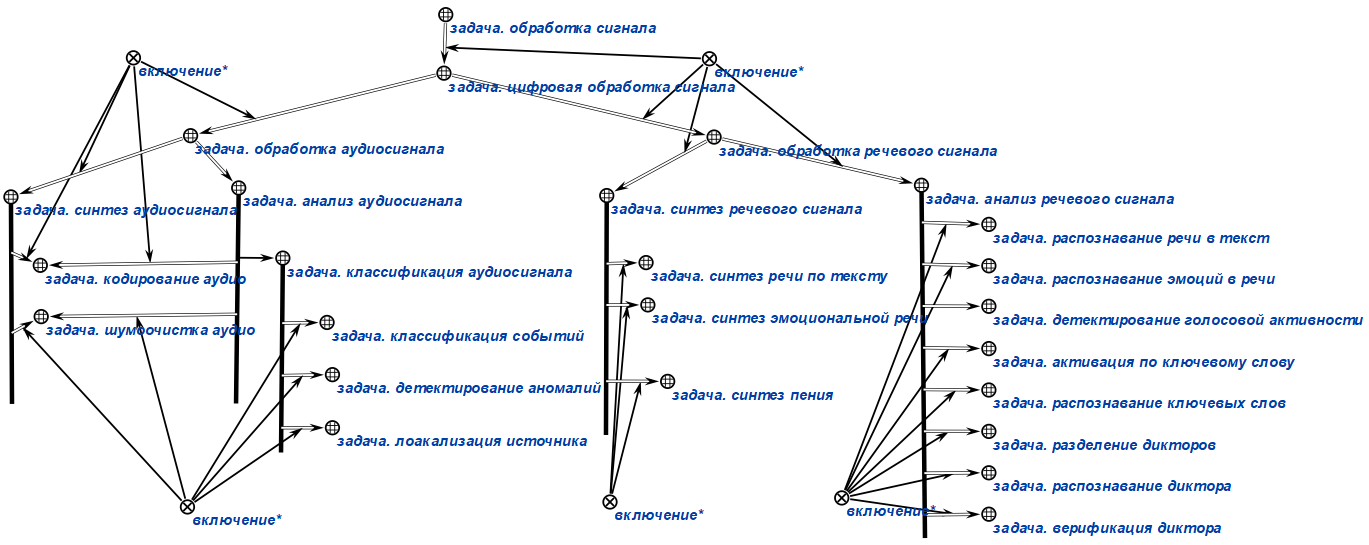
\includegraphics[scale=1.0, width=1.0\textwidth]{author/part4/figures/ch43_fig04_audio-and-speech-tasks-formalization-ru.png}
    }
    \caption{Фрагмент онтологии верхнего уровня задач аудио- и речевых интерфейсов для \textit{интеллектуальных компьютерных систем нового поколения}}
    \label{fig:audio-and-speech-tasks-formalization-ru}
\end{figure}

Описание предметной области моделей сигнала будут более подробно рассмотрены в следующем пункте работы, поэтому не считаем необходимым приводить её здесь.
Онтологию основных характеристик речевого сигнала формализуем в следующем виде (см. \scncite{Laver1994}):

\begin{SCn}
\scnheader{характеристика речевого сигнала}
\begin{scnreltoset}{объединение}
	\scnitem{коммуникативная характеристика}
	\begin{scnindent}
	\scntext{примечание}{кодирует смысл передаваемого сообщения, зависит от намерений отправителя}
	\end{scnindent}
	\scnitem{информативная характеристика}
	\begin{scnindent}
	\scntext{примечание}{кодирует дополнительную информацию передаваемого сообщения, не зависит от намерений отправителя}
	\end{scnindent}
	\scnitem{информативная характеристика}
	\begin{scnindent}
	\scntext{примечание}{кодирует дополнительную информацию передаваемого сообщения, не зависит от намерений отправителя}
	\end{scnindent}
	\scnitem{сегментная характеристика речевого сигнала (Segmantal Features)}
	\begin{scnindent}
	\scntext{примечание}{несет информацию о текущем состоянии источника на протяжении длительности одной или нескольких фонетичесих единиц}
	\end{scnindent}
	\scnitem{надсегментная характеристика речевого сигнала (Suprasegmental Features)}
	\begin{scnindent}
	\scntext{примечание}{несет информацию о состоянии источника и переходах между ними на протяжении времени всего высказывания}
	\end{scnindent}
\end{scnreltoset}
\scnsuperset{лингвистическая характеристика сигнала}
\begin{scnindent}
    \scnhaselement{вербальные средства коммуникации}
    \scnhaselement{коммуникативная характеристика}
    \scntext{определение}{характеристика несущая информацию по средствам использованием системы кодирования человеческого языка}
	\scntext{примечание}{лингвистическая характеристика включают как фонологический код (сегментарный и надсегментный), так и грамматический код (морфологию и синтаксис). Лингвистическая коммуникация информирует получателя о намерениях отправителя с помощью явных словесных форм}
\end{scnindent}
\scnsuperset{паралингвистическая характеристика сигнала}
\begin{scnindent}
    \scnhaselement{невербальные средства коммуникации}
    \scnhaselement{коммуникативная характеристика}
    \scntext{определение}{характеристика несущая информацию посредством  дополнительных средств коммуникации не связанных непосредственно с языком}
    \scntext{примечание}{передает информацию об отношении к предмету разговора, чувствах или эмоциональном состоянии говорящего}
    \begin{scnreltoset}{объединение}
    \scnitem{иинтонация речи}
    \begin{scnindent}
    \begin{scnreltoset}{объединение}
        \scnitem{частота основного тона $F_0$}
        \scnitem{изменение частоты основного тона $\Delta{F_0}$}
    \end{scnreltoset}
    \end{scnindent}
    \scnitem{громкость речи}
    \begin{scnreltoset}{объединение}
        \scnitem{амлитуда сигнала}
        \scnitem{интенсивность сигнала}
    \end{scnreltoset}
    \scnitem{темп речи}
    \scnitem{длительность пауз}
    \end{scnreltoset}
\end{scnindent}
\scnsuperset{экстралингвистическая характеристика сигнала}
\begin{scnindent}
    \scnhaselement{информативная характеристика}
    \scntext{определение}{характеристика, которые не кодируют непосредственно смысл сообщения, но содержит дополнительную информацию об отправителе и условиях коммуникации}
    \scntext{примечание}{передает информацию об отношении к предмету разговора, чувствах или эмоциональном состоянии говорящего}
    \begin{scnreltoset}{объединение}
    \scnitem{характеристика голоса диктора}
    \begin{scnindent}
    \begin{scnreltoset}{объединение}
        \scnitem{высота}
        \scnitem{тембр}
        \scnitem{громоксть}
    \end{scnreltoset}
    \end{scnindent}
    \scnitem{акустическое окружение}
    \end{scnreltoset}
\end{scnindent}
\end{SCn}

Таким образом, представлен результат формализации средствами \textit{SCg-кода} предметной области и онтологии типовых задач аудио и речевых интерфейсов для \textit{интеллектуальных компьютерных систем нового поколения}.

Необходимо отметить, что выше были представлены варианты формализации ключевых понятий области, на основе имеющихся источников информации. Более полные результаты работы по формализации предметной области \textit{аудиоинтерфейса} требуют доступа к закрытым стандартам \textit{AES}, \textit{ISO} и \textit{IEEE}, а также привлечения более широкого круга экспертов, результаты работы с которыми будут фиксироваться в следующих вариантах стандарта и монографии.


\section{Предметная область и онтология моделей параметрического представления сигнала}
\label{sec_audio_interfaces_subject_area_signal_models}

Все вышеперечисленные задачи взаимосвязаны, поскольку относятся к одному и тому же объекту исследования --- \textit{речевому сигналу}. Решение каждой из них непосредственно либо косвенно зависит от эффективности моделирования речи как сложного феномена в различных аспектах: параметрическое представление речевого сигнала и выделение его свойств, моделирование процесса фонации, восприятия и интерпретации содержания речевого сообщения (в том числе фонетического, смыслового, эмоционального). Это делает создание универсальных способов обработки речевых сигналов перспективным научным направлением.
В контексте перечисленных задач моделирование речи можно условно разделить на три уровня: 

\begin{textitemize}
    \item моделирование сигнала в общем виде, используя отсчеты во временной или частотной области; 
    \item моделирование характеристик сигнала, являющихся специфическими для речи и связанных с процессом фонации (таких как частота основного тона, последовательность возбуждения и огибающая амплитудного спектра); 
    \item моделирование высокоуровневых речевых характеристик (голос, акцент, экспрессия, фонетическое и семантическое содержание речевого сообщения).  Каждый следующий уровень основывается на предыдущем и подразумевает использование специальных методов параметрического описания.
\end{textitemize}

К первым двум уровням относятся широко известные в цифровой обработке речевых сигналов модели на основе линейного предсказания, кепстральных коэффициентов и синусоидальных параметров. Отличительные особенности основных типов моделей представлены на рисунке \textit{\nameref{fig:signal-model-types-ru}} 

\begin{figure}[H]
    \centerline{
        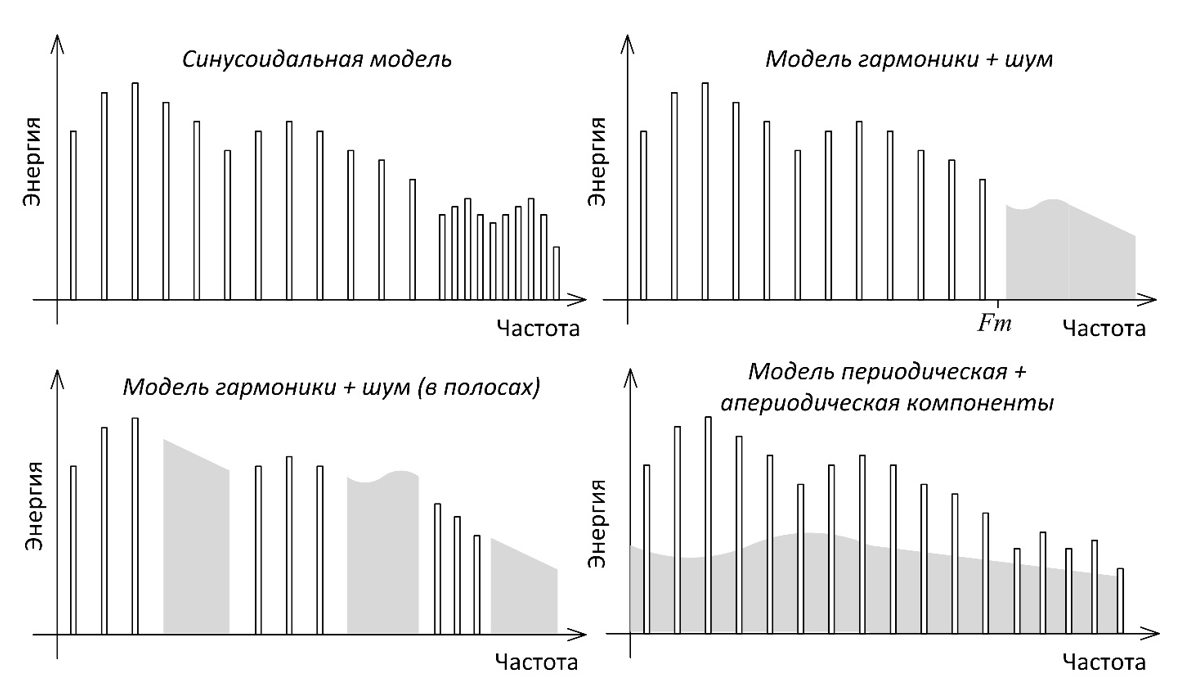
\includegraphics[scale=1.0, width=1.0\textwidth]{author/part4/figures/ch43_fig05_signal-model-types-ru.png}
    }
    \caption{Отличительные особенности  основных типов моделей параметрического представления сигнала}
    \label{fig:signal-model-types-ru}
\end{figure}

Среди подходов, использующих синусоидальное описание сигнала, в настоящее время наиболее перспективными являются смешанные (гибридные) модели, учитывающие возможность разных режимов фонации с участием голосовых связок (вокализованная речь) и без участия голосовых связок (невокализованная речь), причем каждый из этих двух режимов описывается соответствующей моделью. 

Вокализованная речь рассматривается как квазипериодический (детерминистский) сигнал, в то время как невокализованная --- как непериодический (стохастический) сигнал. Наиболее известной среди существующих моделей является модель гармоники+шум, которая используется для решения таких сложных задач, как создание речевых интерфейсов, распознавание речи, синтез речи по тексту, конверсия голоса, шумоподавление, повышение разборчивости и субъективного качества речевых сигналов, коррекция акцента и так далее. Ее преимуществом является теоретическая возможность моделирования вокализованных звуков в виде непрерывных функций с изменяющимися параметрами, что позволяет получить эффективное описание процесса фонации и избежать наложения смежных фрагментов, разрыва фаз при синтезе речи. Недостатком модели является высокая сложность алгоритмов анализа и синтеза, обусловленная нестационарностью речевого сигнала (см. \scncite{Serra1990system}, \scncite{Griffin1988multiband}, \scncite{Petrovsky2011hybrid}, \scncite{Azarov2013instantaneous}). 

Поскольку вокализованная речь состоит из квазипериодических компонент с изменяющимися параметрами, для анализа необходимо использовать цифровые фильтры с изменяющимися характеристиками: их полоса пропускания должна меняться в соответствии с контуром частоты основного тона. Это требует использования специальных частотно-временных преобразований, позволяющих производить оценку периодических составляющих с сильной частотной модуляцией, таких как Фан-Чирп и гармоническое преобразования. Точность оценки параметров непосредственно связана с точностью оценки контура основного тона, поэтому использование надежного и точного способа оценки является необходимым условием для успешного использования данной модели (см. \scncite{Laroche1993hns}, \scncite{Mcaulay1986speech}, \scncite{Degottex2013mixed}). 

Также сложной задачей является автоматическое разделение сигнала на детерминистскую и стохастическую составляющие, для чего используются специальные детекторы периодичности.

Моделирование речевого сигнала на основе линейного предсказания является классическим подходом, который применяется в цифровой обработке речи достаточно продолжительное время. Основным преимуществом модели является раздельное описание сигнала в виде огибающей спектра и сигнала возбуждения. Огибающая спектра определяет фонетику произносимого звука и характеризует состояние речевого тракта, в то время как сигнал возбуждения характеризует состояние голосовых связок и высоту (интонацию) вокализованных звуков. Преимуществом линейного предсказания является также низкая вычислительная сложность. 

Однако, несмотря на это, в последнее время предпочтение отдается моделям, использующим синусоидальное представление сигнала и в первую очередь это касается приложений, подразумевающих синтез речевого сигнала с измененными параметрами, таких как изменение интонации, конверсия голоса, синтез речи по тексту и других. Данный факт можно объяснить тем, что линейное предсказание не обеспечивает эффективных способов для параметрической обработки сигнала возбуждения и непрерывного синтеза выходного сигнала. Каждый речевой фрагмент (кадр) сигнала представляет собой отдельную независимую единицу и при синтезе возникает проблема согласования соседних кадров. Несогласованное изменение огибающей амплитудного и фазового спектра при переходе от кадра к кадру вызывает появление слышимых артефактов. Кроме того, оценка огибающей спектра при помощи классических методов линейного предсказания представляет собой усреднение по всему кадру, вследствие чего ее точность ограничена. Порядок предсказателя определяет сложность модели: для предсказателей низких порядков оценка огибающей спектра получается чрезмерно сглаженной, а для предсказателей высоких порядков точность становится избирательной. Для точек спектра, соответствующих гармоникам основного тона, точность повышается, а для всех остальных точек --- снижается. Оптимальный порядок предсказателя зависит от высоты голоса, но даже в наиболее благоприятном случае точность оценки огибающей спектра имеет погрешность, приводящую к возникновению слышимых искажений.

Использование кепстральных коэффициентов для моделирования речевых сигналов также является классическим подходом. Наиболее хорошо разработанной системой моделирования речевых сигналов, использующей кепстральные коэффициенты, является \textit{TANDEM–STRAIGHT} (см. \scncite{Kawahara2010exploration}, \scncite{Kawahara2009development}). Так же как и для классических способов анализа на основе линейного предсказания, при оценке кепстральных коэффициентов предполагается стационарность сигнала на протяжении интервала наблюдения. Оценка огибающей амплитудного спектра требует сглаживания и также недостаточно точна по сравнению с моделями на основе синусоидальных   \textit{\nameref{fig:straight-spectrum}}.

\begin{figure}[H]
    \centerline{
        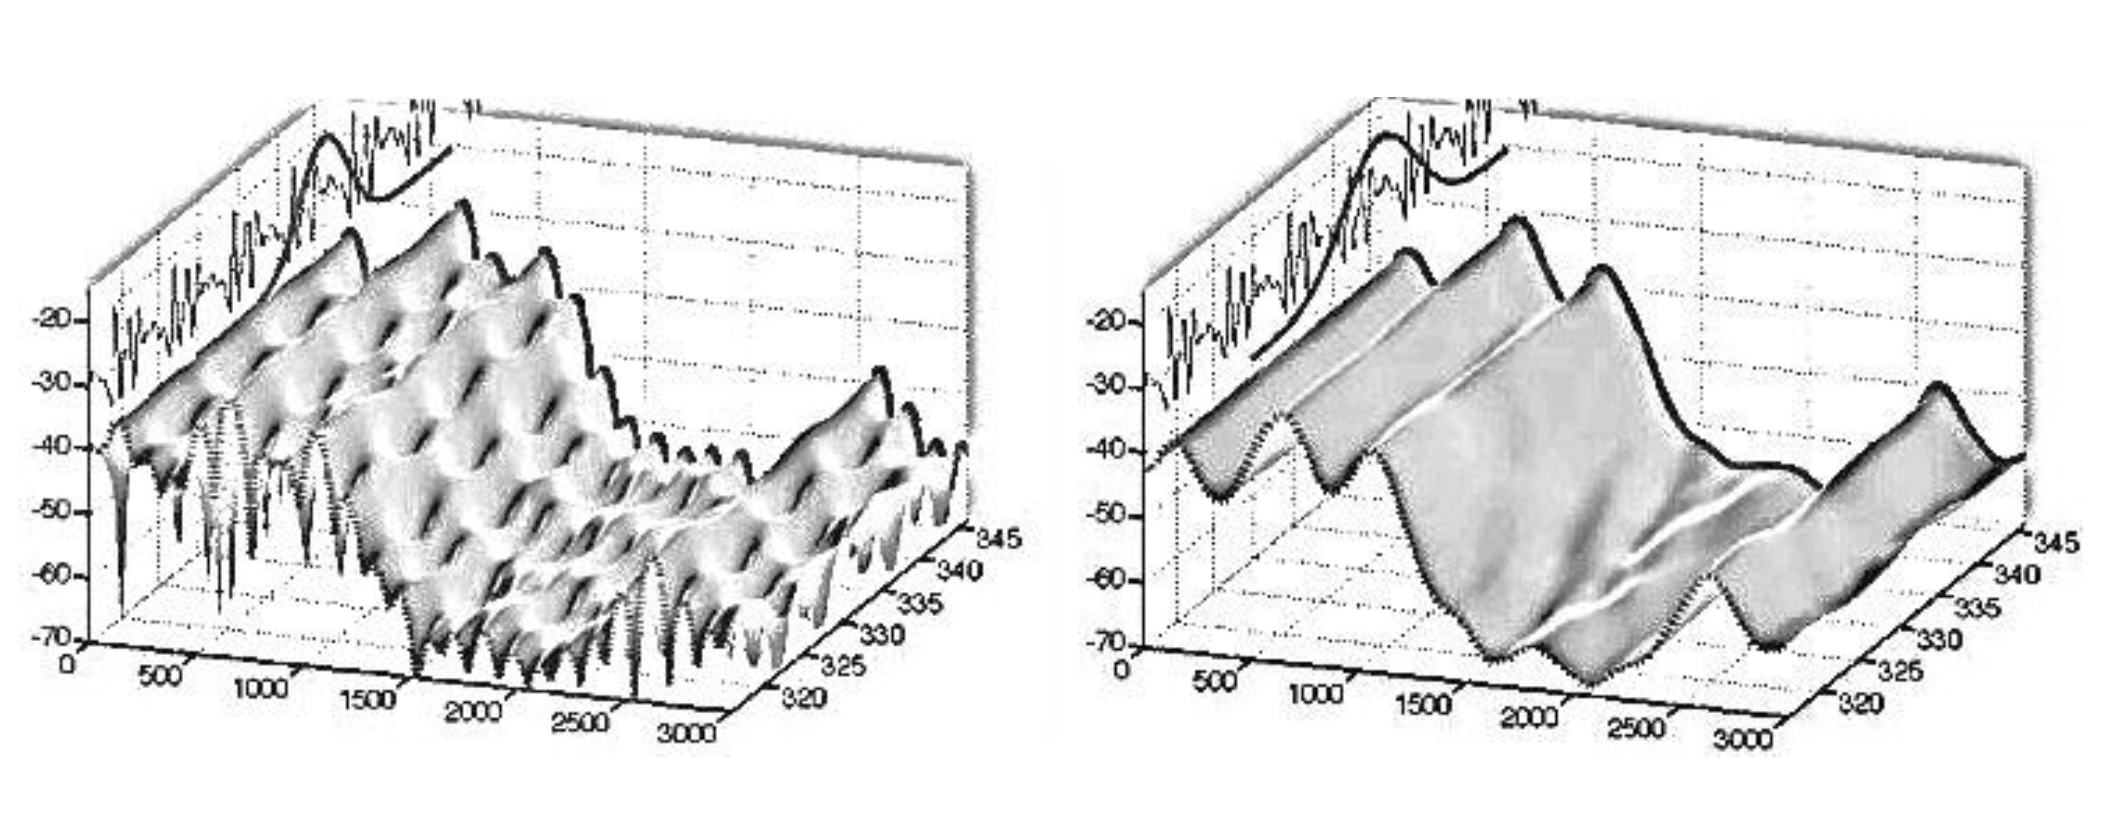
\includegraphics[scale=1.0, width=1.0\textwidth]{author/part4/figures/ch43_fig06_straight-spectrum.png}
    }
    \caption{Спектрограмма сигнала на основе ДПФ (слева) и спектрограмма TANDEM-STRAIGHT (справа)}
    \label{fig:straight-spectrum}
\end{figure}


Благодаря своим широким возможностям гибридная модель на основе синусоидальных параметров является наиболее предпочтительной для использования в большинстве практических случаев. Тем не менее для преодоления существующих ее ограничений, связанных со сложностью оценки параметров, их интерпретации в виде специфических речевых характеристик (параметры речевого тракта, последовательность возбуждения) требуется разработка специальных методов моделирования. 

В зависимости от приложения процесс обработки речевого сигнала с использованием той или иной модели обычно включает анализ (определение параметров модели), модификацию (изменение параметров модели в зависимости от цели приложения) и синтез (формирование нового сигнала из измененных параметров модели). Таким образом, для обеспечения наиболее высокой практической значимости разрабатываемые методы моделирования должны включать средства анализа, обработки параметров и синтеза.

Для решения многих современных прикладных задач требуется не только наличие возможности описания речевого сигнала или процесса фонации, но и использование высокоуровневых речевых характеристик, определяющих персональный голос диктора, экспрессию, фонетику и так далее. К таким задачам относятся конверсия голоса, синтез речи по тексту, верификация диктора и многие другие. Высокоуровневое моделирование речи является очень сложной предметной областью, поскольку требует использования интеллектуальных моделей и методов машинного обучения. На данный момент не существует единого универсального способа, применяемого для разных приложений.

Чтобы подвести итог изложенным в разделе идеям приведем формальное представление некоторых из обозначенных выше концепций:

\begin{SCn}
\scnheader{параметрическая модель сигнала}
\scntext{определение}{математическое выражение, используемое для представления отсчетов сигнала во временной или частотной области}
\scnsuperset{параметрическая модель речевого сигнала}
\begin{scnindent}
    \scntext{определение}{математическое описание характеристик сигнала, являющихся специфическими для речи и связанных с процессом фонации (таких как частота основного тона, последовательность возбуждения и огибающая амплитудного спектра)}
    \scntext{примечание}{к основным моделям речевого сигнала относят: модели на основе линейного предсказания; на основе кепстрального представления; синусоидальные и гибридные модели. Среди гибридных моделей наиболее известна модель гармоники+шум}
\end{scnindent}
\end{SCn}

Подавляющее большинство высокоуровневых речевых моделей, используемых на практике, являются проблемно-ориентированными и могут применяться только для решения одной, узкоспециализированной задачи. Поэтому критически важным является факт того, чтобы в \textit{базе знаний} \textit{интеллектуальной компьютерной системы} содержалось достаточно информации для определения подходящего типа модели представления сигнала и активации соответствующего \textit{агента} в рамках \textit{многоагентной системы} в зависимости от класса м модели решаемой задачи. Более подробно соответствующие понятия рассмотрены в рамках \textit{Главы \ref{chapter_actions}}


\section*{Заключение к \textit{Главе \ref{chapter_audio_interfaces}~\nameref{chapter_audio_interfaces}}}

В главе изложены идеи, лежащие в основе оригинального подхода к проектированию аудиоинтерфейсов \textit{интеллектуальных компьютерных систем} на основе онтологического проектирования и формализации системы понятий из соответствующей предметной области, с использованием Технологии OSTIS. Изложены основные принципы лежащие в основе данного подхода, а также их отличительные особенности от общепринятых.

К ограничениям предлагаемого подхода можно отнести следующие основные факторы. Очевидно, что для достижения поставленной цели и реализации задач по формализации любой предметной области, в том числе и аудиоинтерфейсов, требуется в первую очередь большое количество источников знаний для их пополнения. Для преодоления данной проблемы требуется привлечение большого количества экспертов, обладающих соответствующими компетенциями и знаниями в предметной области, либо же разработка механизмов надежного автоматического извлечения этих знаний из имеющихся источников.

Прямой доступ к знаниям экспертов весьма ограничен, поскольку это требует значимых усилий по подбору репрезентативной выборки таких экспертов, выстраиванию эффективных и интероперабельных взаимоотношений между сторонами процесса, что зачастую зависит от большого количества субъективных факторов, --- соответственно, требует большого количества временных и материальных ресурсов.

Известно, что существенное количество информации, накопленной человечеством, хранится в виде текстов на естественных языках. Процесс извлечения данной информации и представления её в формализованном виде --- в виде знаний, также выглядит нетривиальным.
 
Исходя из природы данных проблем, по мнению авторов, видятся следующие основные направления их преодоления и, как следствие, две основные стратегии развития предложенного подхода.

\begin{enumerate}
  \item Создание для экспертов, работающих в домене аудио и речевых интерфейсов, специализированных инструментальных средств по формализации и представлению знаний из данной предметной области, фиксации их в виде стандартов единой формы. Подобные инструменты должны обладать качественно новыми функциональными возможностями, обеспечивающими высокий уровень совместимости и интероперабельности в процессе накопления и стандартизации знаний, чтобы сами эксперты были заинтересованы в применении и широком распространении данной технологии для представления знаний. Данный пункт является одной из ключевых задач \textit{Технологии OSTIS} и \textit{Стандарта OSTIS}.
  \item Создание автоматизированных и автоматических средств извлечения знаний из существующих источников информации, в первую очередь текстов на естественном языке. К видам документов, в которых содержится уже структурированная и отчасти формализованная информация, относятся в первую очередь: стандарты, протоколы, рекомендации (RFC), инструкции и т.д. Следовательно процесс автоматизации извлечения знаний должен быть направлен в первую очередь на формализацию уже существующих отраслевых стандартов разработки аудиоинтерфейсов, систем обработки и кодирования аудиоинформации, систем обработки речевых сигналов, таких как стандарты серии \textit{ISO}, \textit{IEEE} и \textit{AES} (Audio Engineering Society): \scncite{ISO14496-3}, \scncite{ISO23003-3}, \scncite{IEEE1857-8}, \scncite{IEC62087-2}, \scncite{AES3250}.
\end{enumerate}

Реализация подхода, предложенного в данной главе, позволит обеспечить свойства унификации, семантической совместимости и интероперабельности, при разработке аудио и речевых интерфейсов (своеобразный аналог \textit{Модели OSI/ISO} в области проектирования \textit{интерфейсов} \textit{интеллектуальных компьютерных систем}), что в итоге позволит существенным образом сократить издержки при создании интеллектуальных компьютерных систем нового поколения для решении сложных комплексных задач.


%\input{author/references}